\documentclass{beamer}
\usepackage[utf8]{inputenc}

\title{Project 2}
\subtitle{Data Analysis of Monte Carlo Simulation of InGaAs Semiconductor Device}
\author{Michael Brunetti}
\institute{
EECE 5090 -- Linear Systems Analysis\\
UMass Lowell}
\date{June 11, 2019}
 
 
 
\begin{document}
 
\frame{\titlepage}

\begin{frame}{Strategy}
    \begin{itemize}
        \item Build on previous work -- use least squares curve fit parameters from Project 1.
        \item Characterize and model steady-state I-V relationship for 3 devices.
        \item Analyze oscillation frequency vs voltage relationship. Develop a model if possible.
    \end{itemize}
\end{frame}

\begin{frame}{Steady-State I-V Curve -- Device 1}
    \begin{figure}
        \centering
        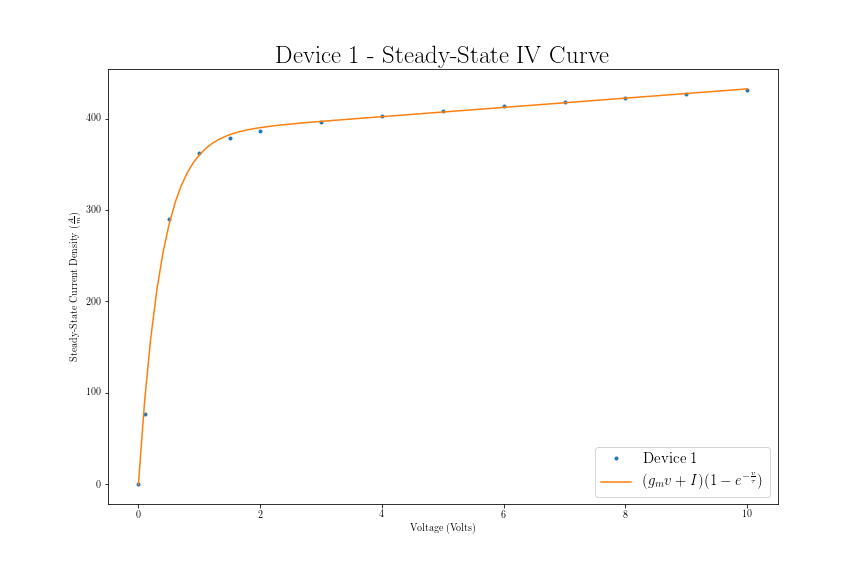
\includegraphics[scale=0.35]{Figures/Device_1/SteadyState_fit.png}
        \label{fig:dev1_ss}
    \end{figure}
\end{frame}

\begin{frame}{Steady-State I-V Curve -- Device 1}
    \begin{itemize}
        \item Model function: $ i = \left( g_m v + I_{sat} \right) \left( 1 - e^{-\frac{v}{\tau}} \right) $
        \item Exponential rise to saturation, followed by linear IV relationship
        \item $g_m = 5.06 \frac{\textnormal{A}}{\textnormal{m} \cdot \textnormal{V}}$ -- ``transconductance gain"
        \item $I_{sat} = 382 \frac{\textnormal{A}}{\textnormal{m}}$ -- ``zero voltage saturation current"
        \item $\tau = 0.374 \textnormal{V}$ -- ``exponential decay constant"
    \end{itemize}
\end{frame}

\begin{frame}{Steady-State I-V Curve -- Device 2}
    \begin{figure}
        \centering
        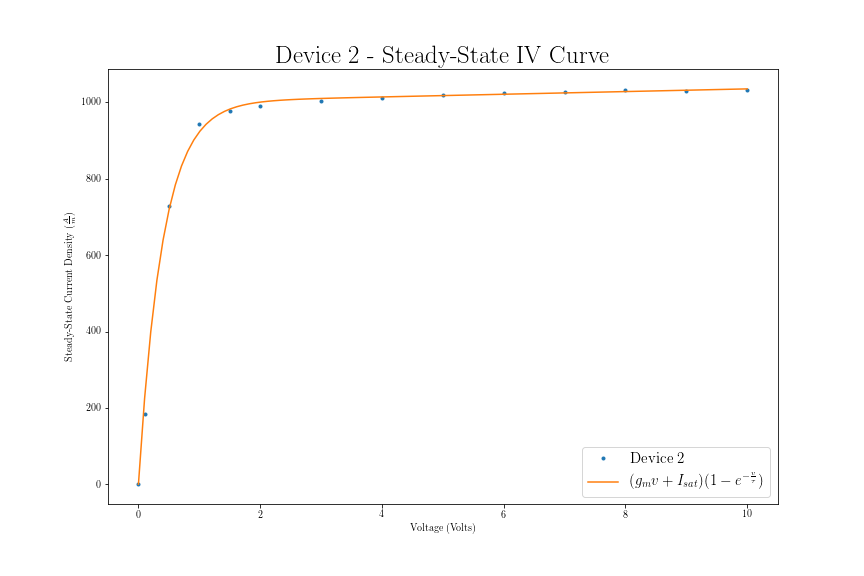
\includegraphics[scale=0.35]{Figures/Device_2/SteadyState_Fit.png}
        \label{fig:dev2_ss}
    \end{figure}
\end{frame}

\begin{frame}{Steady-State I-V Curve -- Device 2}
    \begin{itemize}
        \item Model function: $ i = \left( g_m v + I_{sat} \right) \left( 1 - e^{-\frac{v}{\tau}} \right) $
        \item Exponential rise to saturation, followed by linear IV relationship
        \item $g_m = 3.51 \frac{\textnormal{A}}{\textnormal{m} \cdot \textnormal{V}}$ -- ``transconductance gain" 
        \item $I_{sat} = 1000 \frac{\textnormal{A}}{\textnormal{m}}$ -- ``zero voltage saturation current"
        \item $\tau = 0.398 \textnormal{V}$ -- ``exponential decay constant"
    \end{itemize}
\end{frame}

\begin{frame}{Steady-State I-V Curve -- Device 3}
    \begin{figure}
        \centering
        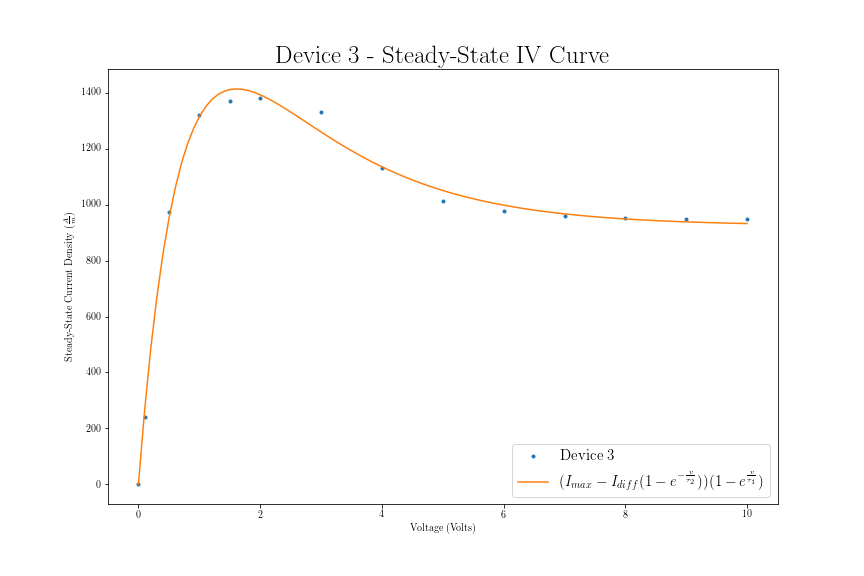
\includegraphics[scale=0.35]{Figures/Device_3/SteadyState_Fit.png}
        \label{fig:dev3_ss}
    \end{figure}
\end{frame}

\begin{frame}{Steady-State I-V Curve -- Device 3}
    \begin{itemize}
        \item Model function: $ i = \left( I_{max} - I_{diff} \left( 1 - e^{\frac{v}{\tau_2}} \right) \right) \left( 1 - e^{\frac{v}{\tau_1}} \right)$
        \item $I_{max} - I_{diff} = \lim_{v\to\infty} i = 927 \frac{\textnormal{A}}{\textnormal{m}}$
        \item $\tau_1 = 0.772 \textnormal{V}$ -- ``exponential decay constant for rise"
        \item $\tau_2 = 1.75 \textnormal{V}$ -- ``exponential decay constant for drop"
        \item $\tau_1 < \tau_2$
    \end{itemize}
\end{frame}

\begin{frame}{Natural Frequency vs Drain-Source Voltage -- Device 1}
    \begin{figure}
        \centering
        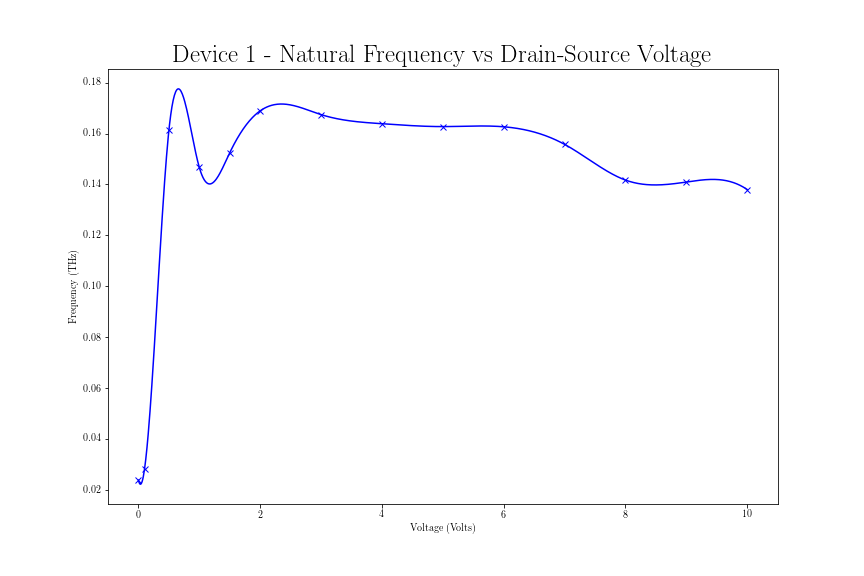
\includegraphics[scale=0.35]{Figures/Device_1/NaturalFrequency.png}
        \label{fig:nfreq_1}
    \end{figure}
\end{frame}

\begin{frame}{Natural Frequency vs Drain-Source Voltage -- Device 2}
    \begin{figure}
        \centering
        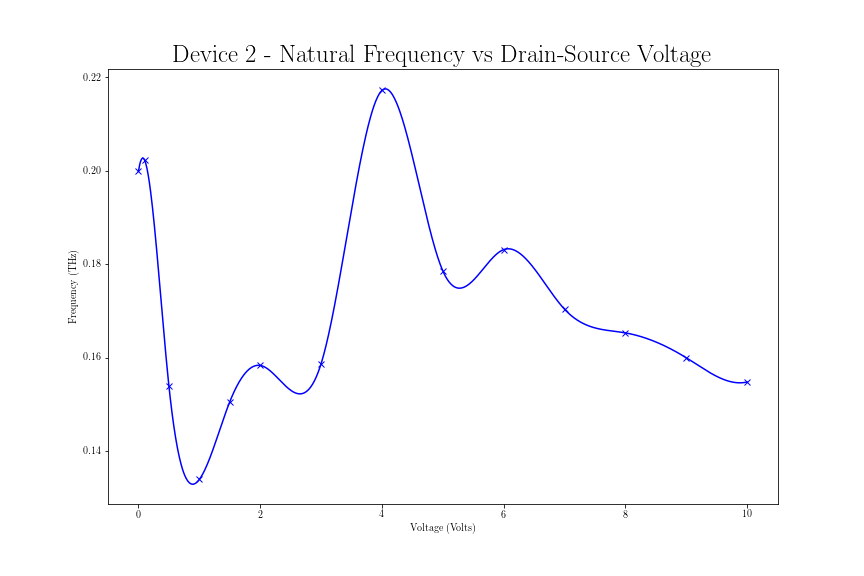
\includegraphics[scale=0.35]{Figures/Device_2/NaturalFrequency.png}
        \label{fig:nfreq_2}
    \end{figure}
\end{frame}

\begin{frame}{Natural Frequency vs Drain-Source Voltage -- Device 3}
    \begin{figure}
        \centering
        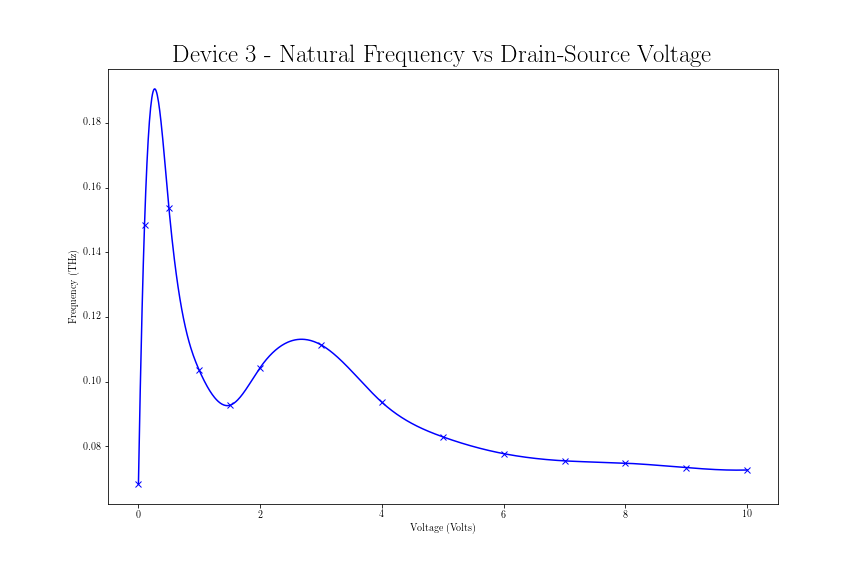
\includegraphics[scale=0.35]{Figures/Device_3/NaturalFrequency.png}
        \label{fig:nfreq_3}
    \end{figure}
\end{frame}
 
\end{document}